\documentclass{beamer}
\usepackage[utf8]{inputenc}
\usepackage{amsmath}
\usepackage{graphicx}
\usepackage{xcolor}
\usepackage{tikz}

\usetheme{Madrid}
\usecolortheme{default}

% Define custom colors inspired by Star Trek DS9
\definecolor{ds9blue}{RGB}{25,25,112} % Midnight Blue
\definecolor{ds9gold}{RGB}{218,165,32} % Goldenrod
\definecolor{ds9grey}{RGB}{105,105,105} % Dim Gray
\definecolor{ds9red}{RGB}{178,34,34} % Firebrick

% Customize the colors
\setbeamercolor{title}{fg=ds9gold}
\setbeamercolor{frametitle}{bg=ds9blue, fg=white}
\setbeamercolor{block title}{bg=ds9gold, fg=black}
\setbeamercolor{block body}{bg=ds9grey!20, fg=black}
\setbeamercolor{section in toc}{fg=ds9gold}
\setbeamercolor{subsection in toc}{fg=ds9gold!70}
\setbeamercolor{footline}{bg=ds9blue, fg=white}
\setbeamercolor{author in head/foot}{fg=white}
\setbeamercolor{date in head/foot}{fg=white}
\setbeamercolor{title in head/foot}{fg=white}

% Title page configuration
\title[Acceleration and Motion]{PHYS11 CH3:}
\subtitle{ Acceleration and Motion}
\author[Mr. Gullo]{Mr. Gullo}
\date[Sept 2024]{September 2024}

% Table of contents at the beginning of each section
\AtBeginSection[]
{
  \begin{frame}
    \frametitle{Table of Contents}
    \tableofcontents[currentsection]
  \end{frame}
}
\begin{document}

\frame{\titlepage}

\begin{frame}
\frametitle{Introduction}
\begin{itemize}
    \item Understanding motion is crucial in physics
    \item Acceleration: a fundamental concept
    \item Key topics:
    \begin{itemize}
        \item Average acceleration
        \item Kinematic equations
        \item Graphical analysis
        \item Vector directions
    \end{itemize}
\end{itemize}
\end{frame}

\begin{frame}
\frametitle{Acceleration: Definition}
\begin{itemize}
    \item Acceleration: rate of change of velocity with time
    \item Vector quantity (magnitude and direction)
    \item Formula:
    \[\vec{a} = \frac{\Delta \vec{v}}{\Delta t}\]
    where:
    \begin{itemize}
        \item $\vec{a}$ is acceleration
        \item $\Delta \vec{v} = \vec{v} - \vec{v}_0$ is change in velocity
        \item $\Delta t = t - t_0$ is change in time
    \end{itemize}
\end{itemize}
\end{frame}

\begin{frame}
\frametitle{Average Acceleration}
\begin{itemize}
    \item Average acceleration over a time interval:
    \[\vec{a}_{\text{avg}} = \frac{\vec{v} - \vec{v}_0}{t - t_0}\]
    \item Useful for calculating overall change in motion
\end{itemize}
\end{frame}

\begin{frame}
\frametitle{Kinematic Equations for Uniform Acceleration}
For constant acceleration:
\begin{align*}
\vec{v} &= \vec{v}_0 + \vec{a}t \\
\vec{x} &= \vec{x}_0 + \vec{v}_0 t + \tfrac{1}{2} \vec{a} t^2 \\
v^2 &= v_0^2 + 2a (x - x_0)
\end{align*}
where:
\begin{itemize}
    \item $\vec{v}$: final velocity
    \item $\vec{v}_0$: initial velocity
    \item $\vec{a}$: acceleration
    \item $t$: time
    \item $\vec{x}$: final position
    \item $\vec{x}_0$: initial position
\end{itemize}
\end{frame}

\begin{frame}
\frametitle{Graphical Analysis: Velocity vs. Time}
\begin{itemize}
    \item Slope represents acceleration
    \item Straight line: constant acceleration
    \item Curved line: changing acceleration
\end{itemize}
\end{frame}

\begin{frame}
\frametitle{Graphical Analysis: Displacement vs. Time}
\begin{itemize}
    \item Slope represents velocity
    \item Straight line: constant velocity (zero acceleration)
    \item Curved line: changing velocity (non-zero acceleration)
\end{itemize}
\end{frame}

\begin{frame}
\frametitle{Vectors and Direction}
\begin{itemize}
    \item Acceleration, velocity, and displacement are vector quantities
    \item Direction is significant:
    \begin{itemize}
        \item Positive acceleration: vector points in positive direction
        \item Negative acceleration: vector points in negative direction
        \item Positive and negative vectors are 180° apart
    \end{itemize}
    \item \textbf{Important note:} We use "negative acceleration" instead of "deceleration"
    \begin{itemize}
        \item This emphasizes that acceleration is a vector quantity
        \item It reinforces the concept that slowing down is just acceleration in the opposite direction
        \item Helps avoid misconceptions about the nature of acceleration
    \end{itemize}
\end{itemize}
\end{frame}

\begin{frame}
\frametitle{Example 1: Calculating Average Acceleration}
Problem: Velocity increases from 0 to 20 m/s in 10 s. What is the average acceleration?

Solution:
\begin{align*}
\vec{a}_{\text{avg}} &= \frac{\vec{v} - \vec{v}_0}{t} \\
&= \frac{20 \, \text{m/s} - 0 \, \text{m/s}}{10 \, \text{s}} \\
&= 2 \, \text{m/s}^2
\end{align*}

Answer: The average acceleration is $2 \, \text{m/s}^2$.
\end{frame}

\begin{frame}
\frametitle{Example 2: Interpreting Velocity vs. Time Graphs}
Problem: Show that the acceleration of a jet car is $5.0 \, \text{m/s}^2$ at any point on the graph.

\begin{figure}[H]
    \centering
    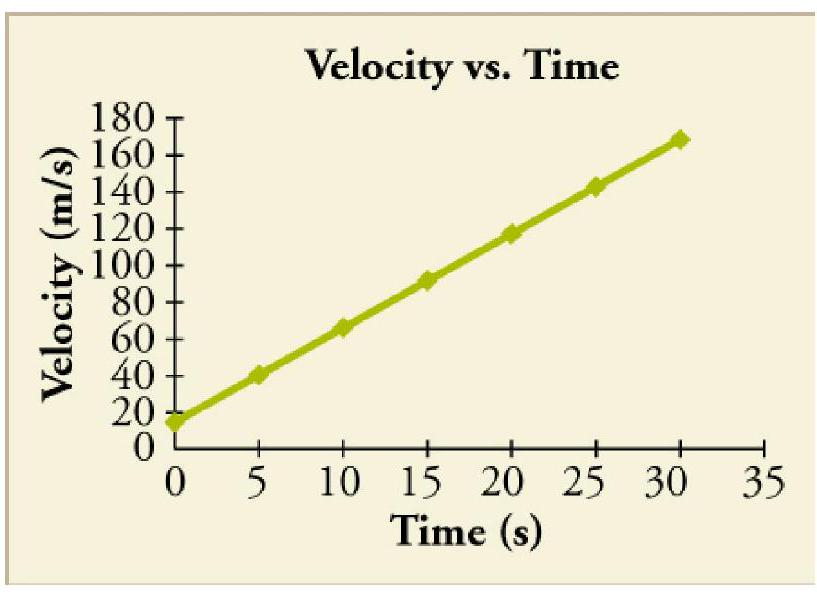
\includegraphics[width=0.75\linewidth]{2024_09_22_d75bb9ada91612339d1ag-12.jpg}
\caption{Velocity vs. Time Graph for a Jet Car}
\end{figure}

\end{frame}

\begin{frame}
\begin{figure}[H]
    \centering
    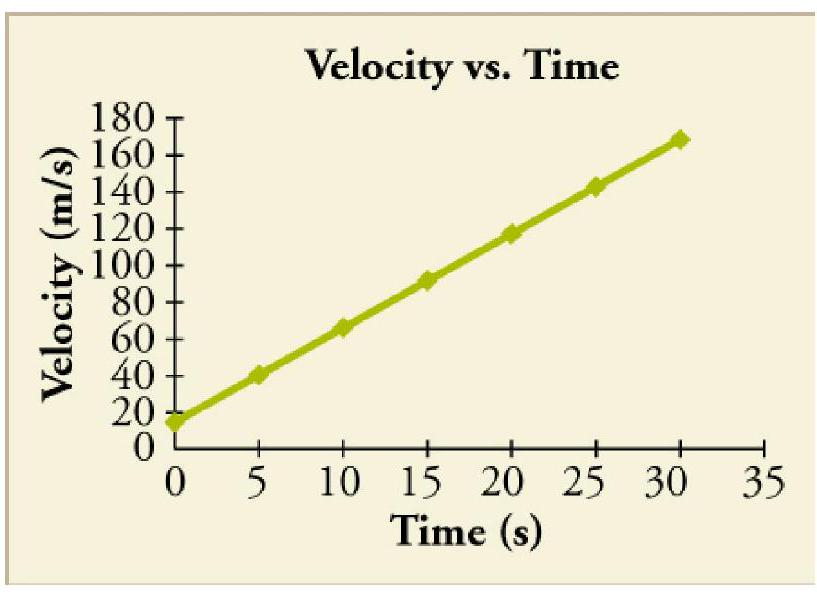
\includegraphics[width=0.5\linewidth]{2024_09_22_d75bb9ada91612339d1ag-12.jpg}
\caption{Velocity vs. Time Graph for a Jet Car}
\end{figure}
\begin{itemize}
    \item Slope of v-t graph represents acceleration
    \item Straight line indicates constant acceleration
    \item Slope = $\frac{\Delta \vec{v}}{\Delta t} = \frac{\vec{v}}{t} = 5.0 \, \text{m/s}^2$
\end{itemize}

Answer: The acceleration is $5.0 \, \text{m/s}^2$ at any point on the graph.
\end{frame}
\begin{frame}
\frametitle{Car Acceleration Problem: Two-Phase Motion}
\textbf{Problem Statement:}
A car undergoes two-phase motion:
\begin{itemize}
\item Phase 1: Accelerates from rest at $3.0 , \text{m/s}^2$ to $21.0 , \text{m/s}$
\item Phase 2: Decelerates at $4.0 , \text{m/s}^2$ until stopping
\end{itemize}
\vspace{0.5cm}
\textbf{Question:} Find the total time of travel.
\end{frame}
\begin{frame}
\frametitle{Solution: Total Time and Visualization}
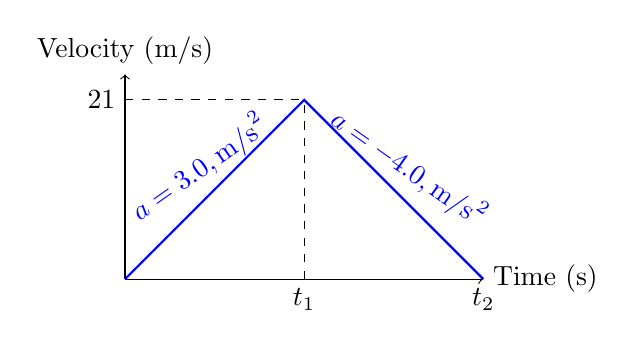
\begin{tikzpicture}[scale=0.65]
\draw[->] (0,0) -- (7,0) node[right] {Time (s)};
\draw[->] (0,0) -- (0,4) node[above] {Velocity (m/s)};
\draw[thick, blue] (0,0) -- (3.5,3.5) -- (7,0);
\draw[dashed] (3.5,0) -- (3.5,3.5);
\draw[dashed] (0,3.5) -- (3.5,3.5);
\node[left] at (0,3.5) {21};
\node[below] at (3.5,0) {$t_1$};
\node[below] at (7,0) {$t_2$};
\node[above, blue, rotate=35] at (1.75,1.75) {$a = 3.0 , \text{m/s}^2$};
\node[above, blue, rotate=-35] at (5.25,1.75) {$a = -4.0 , \text{m/s}^2$};
\end{tikzpicture}
\end{frame}
\begin{frame}
\frametitle{Solution: Phase 1 - Acceleration}
\textbf{Phase 1 (Acceleration):}
\begin{itemize}
\item Initial velocity: $v_0 = 0 , \text{m/s}$
\item Final velocity: $v = 21.0 , \text{m/s}$
\item Acceleration: $a = 3.0 , \text{m/s}^2$
\end{itemize}
Using the equation: $v = v_0 + at_1$
\begin{align*}
21 &= 0 + 3t_1 \
t_1 &= \frac{21}{3} = 7.0 , \text{s}
\end{align*}
\textbf{Time for Phase 1: $7.0 , \text{s}$}
\end{frame}
\begin{frame}
\frametitle{Solution: Phase 2 - Deceleration}
\textbf{Phase 2 (Deceleration):}
\begin{itemize}
\item Initial velocity: $v_0 = 21.0 , \text{m/s}$
\item Final velocity: $v = 0 , \text{m/s}$
\item Deceleration: $a = -4.0 , \text{m/s}^2$
\end{itemize}
Using the equation: $v = v_0 + at_2$
\begin{align*}
0 &= 21 + (-4)t_2 \
4t_2 &= 21 \
t_2 &= \frac{21}{4} = 5.25 , \text{s}
\end{align*}
\textbf{Time for Phase 2: $5.25 , \text{s}$}

\textbf{Total time:}
\begin{align*}
t_{\text{total}} &= t_1 + t_2 \
&= 7.0 , \text{s} + 5.25 , \text{s} \
&= 12.25 , \text{s}
\end{align*}
\textbf{Answer:} The total time of travel is $12.25 , \text{s}$ (approximately $12 , \text{s}$)


\end{frame}

\begin{frame}
\frametitle{Conclusion}
\begin{itemize}
    \item Understanding acceleration is essential in physics
    \item Key concepts covered:
    \begin{itemize}
        \item Definition of acceleration
        \item Average acceleration
        \item Kinematic equations
        \item Graphical analysis
        \item Vector directions
    \end{itemize}
    \item These concepts help analyze real-world situations
    \item Practice with examples to master the material
    \item Remember: "Negative acceleration" instead of "deceleration" emphasizes the vector nature of acceleration
\end{itemize}
\end{frame}

\end{document}